El Modelo Estándar (\ME) describe la composición del universo usando 6 quarks, 6 leptones y algunas partículas portadoras de las cuatro  fuerzas (o interacciones) conocidas, cada una mediada por una partícula fundamental, ellas son los fotones $\mathbf{\gamma}$ (interacción electromagnética), los higgs $\mathbf{H}$ (interacción gravitatoria), los gluones $\mathbf{g}$ (interacción fuerte) y las partículas $\mathbf{W}$ y $\mathbf{Z}$ (fuerza débil). Actualmente la Gravedad está incluida solamente en el Modelo Estándar como hipótesis especulativa, pues los bosones higgs no se han observados directamente aún.

Las partículas elementales están divididas en dos categorías según el valor de su espín en \fermiones ~ (espín semi-entero, para elementales $1/2$) y \bosones ~ (espín entero, para elementales $1$ menos el higss con $0$), estos obedecen también a la \fermidirac ~ y la \boseeinstein, respectivamente, solo cumpliendo el \pauli ~ los primeros.

\begin{figure}
    \centering
    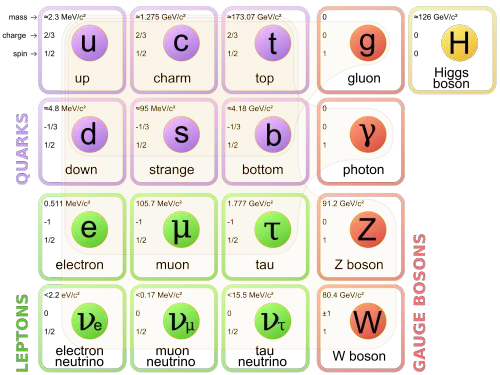
\includegraphics[width=0.49\textwidth]{Fisica_de_Particulas/imagenes/standard_model.png}
    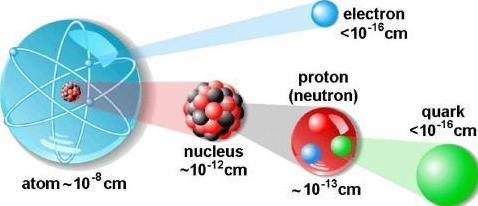
\includegraphics[width=0.49\textwidth]{Fisica_de_Particulas/imagenes/atom.jpg}
    \caption{Clasificación de las partículas según el modelo estándar de las partículas elementales}
    \label{estandar}
\end{figure}

Como se observa en la Fig. \ref{estandar} los \fermiones ~ est\'an a la vez divididos en dos subgrupos importantes (\quarks ~ y \leptones), estos con claras diferencias palmeables:
\begin{itemize}
\item[-] \textbf{Carga :} los \leptones ~poseen carga eléctrica neutra (los neutralinos) o una carga fundamental unidad (electrón, muón y tau), los quarks, por otra parte, disponen de cargas fraccionadas ($- 1/3$ o $+ 2/3$). 
\item[-] \textbf{Fuerzas :} la fuerza fuerte mediada por sus partículas portadoras los gluones \textbf{g} mantiene unido los núcleos atómicos y solo act\'ua sobre los quarks raz\'on por la cual no existirán nunca libremente en la naturaleza, esta fuerza adem\'as aumenta a medida que se mueven los quarks entre sí, asegurando que un quark libre nunca se detecte. 
\end{itemize}

\subsection*{Los \Quarks}

El campo de estudio dedicado a las interacciones entre quarks y gluones se llama Cromodinámica Cuántica (\QCD), en concreto explica la interacci\'on entre los quarks mediante el intercambio de gluones que son los portadores de un nuevo n\'umero cu\'antico (el color el cual fue introducido por Greenberg en 1964 para
restaurar el principio de Pauli) para formar todas las part\'iculas que interaccionan fuertemente (hadrones), ya sean mesones donde interaccionan quark y antiquark, \textbf{q\={q}}, o bariones
donde interaccionan tres quarks de diferente color, \textbf{qqq} dado que los quarks son part\'iculas de esp\'in semi-entero, dos quarks del mismo tipo no pod\'ian tener los mismos n\'umeros cu\'anticos. 

Ejemplos de bariones:
\begin{itemize}
\item[-] \href{https://es.wikipedia.org/wiki/Bari\%C3\%B3n_delta}{\textbf{Los delta :}} también llamados resonancias delta son bariones relativamente ligeros $(1.232\pm 1)$ MeV/c$^2$, están compuestos por un \quark ~ arriba \textbf{u} y un \quark ~ abajo \textbf{d}. Algunas partículas que forma parte de está familia son $\Delta^{++}$, $\Delta^{+}$, $\Delta^{-}$, $\Delta^{0}$, compuestos por \textbf{uuu}, \textbf{uud}, \textbf{udd} y \textbf{ddd}, respectivamente.

\item[-] \href{https://es.wikipedia.org/wiki/Bari\%C3\%B3n_lambda}{\textbf{Los lambda :}} está compuesto por un quark arriba \textbf{u}, uno abajo \textbf{d} y todas las combinaciones con los quark restantes. Las partículas que forman parte de la familia son $\wedge^0$, $\wedge^+_c$, $\wedge^0_b$ y $\wedge^+_t$, compuestos por \textbf{uds}, \textbf{udc}, \textbf{udb} y , \textbf{udt}, respectivamente. 

%\item[-] \href{https://es.wikipedia.org/wiki/Bari\%C3\%B3n_sigma}{\textbf{Los sigma :}}
\item[-] \href{https://es.wikipedia.org/wiki/Bari\%C3\%B3n_xi}{\textbf{Los xi :}} está compuesto por tres \quarks : un \quark ~ arriba (\textbf{u}) o abajo (\textbf{d}) y dos \quarks ~ más pesados. Estas partículas son inestables, que les lleva a desintegrarse rápidamente en partículas más ligeras a través de una cadena de desintegraciones. Las partículas que forman parte de la familia $\Xi^i_{abc}$ donde $i=\{++,~ +,~ -,~ 0\}$, algunos ejemplos son $\Xi^0$, $\Xi^-$, $\Xi^+_{c}$, $\Xi^0_{c}$, compuestos por la combinación de \quarks ~ \textbf{uss}, \textbf{dss}, \textbf{usc}, \textbf{dsc}, respectivamente.

\item[-] \href{https://es.wikipedia.org/wiki/Bari\%C3\%B3n_omega}{\textbf{El omega negativo :}} son una familia de partículas que no poseen ningún \quark ~ arriba (\textbf{u}) o \quark ~ abajo (\textbf{d}), además el Modelo Estándar teoriza la inexistencia con de combinaciones que contengan \quarks ~ cima \textbf{t}. Las familias que forman parte de la familia son $\Omega^i_{abc}$ donde $i=\{++,~ +,~ -,~ 0\}$ relacionado con la respectiva carga resultante, algunos ejemplos son $\Omega^-$, $\Omega^0_c$, $\Omega^-_{bb}$, $\Omega^-0_{cbb}$, compuestos por la combinación quarks \textbf{sss}, \textbf{css}, \textbf{sbb}, \textbf{cbb}, respectivamente.

\item[-] \href{https://es.wikipedia.org/wiki/Bari\%C3\%B3n_omega}{\textbf{El neutrón ($N^0$) :}} es incluida en la definición de nucleones ya que conforman el núcleo de los átomos, es una partícula subatómica sin carga neta,  de la \QCD ~ se define que es partícula compuesta por la unión estable de quarks \textbf{udd}.

\item[-] \href{https://es.wikipedia.org/wiki/Prot\%C3\%B3n}{\textbf{El protón ($p^+$) :}} es incluida en la definición de nucleones ya que conforman el núcleo de los átomos, es una partícula subatómica con una carga eléctrica elemental positiva, de la \QCD ~ se define que es partícula compuesta por la unión estable \textbf{uud}.

\end{itemize}
hay una regla extra para todos los sub-índices \textit{abc}, no se incluye el símbolo correspondiente al \quark ~\textbf{s}, y con la regla que forma parte de la definición del barión referido sumado al valor de la carga incluida en el supra-índice $i$ es inducible la inclusión de los \quarks ~ \textbf{u} y \textbf{d}, de esta forma lógica se reconstruye de forma únivoca la simbología anteriormente descrita %del barión y los \quarks ~ que los incluye
. Todas partículas anteriormente conformadas se pueden distinguir por su carga eléctrica, y cada una posee una respectiva antipartícula con carga opuesta, formadas por sus correspondientes antiquarks.

Ejemplos de mesones son:
\begin{itemize}
\item[-] \href{https://es.wikipedia.org/wiki/Pion}{\textbf{El pión :}} son la familia $\pi^i$ donde $i=\{+, ~ -,~0\}$ está compuesto por un quark y un antiquark, siendo y es el más ligero de todo el grupo, de manera general son muy inestables. Las partículas que forman parte de su familia son $\pi^+$, $\pi^-$ y $\pi^0$, compuestos por los \quarks ~ \textbf{u\={d}}, \textbf{d\={u}} y \textbf{u\={u}}/\textbf{d\={d}}, respectivamente.

\item[-] \href{https://es.wikipedia.org/wiki/Ka\%C3\%B3n}{\textbf{El kaon :}} es de la familia $K$ estos contienen dos quarks, siendo uno de ellos un quark o antiquark extraño. Las part\'iculas que forman parte de la familia son $K^+$, $K^0$, $K^0_S$ y $K^0_L$, compuestos por los quark \textbf{u\={s}}, \textbf{d\={s}}, \textbf{[d\={s} - s\={d}]}/$\mathbf{\sqrt{2}}$, \textbf{[d\={s} + s\={d}]}/$\mathbf{\sqrt{2}}$, respectivamente.

\item[-] \href{https://es.wikipedia.org/wiki/Mes\%C3\%B3n_rho}{\textbf{El rho :}} son una familia de partículas de corta vida, estos pueden ser interpretados como un estado ligado de un \quark ~ y un anti-\quark ~, siendo una versión excitada de un \href{https://es.wikipedia.org/wiki/Pion}{pión}, su diferencia radica en el valor de su espín entero (un mesón vectorial). Las part\'iculas que forman parte de la familia son $\rho^+$, $\rho^-$ y $\rho^0$ compuestos por los quarks \textbf{u\={d}}, \textbf{d\={u}}, \textbf{[u\={u} - d\={d}]}/$\mathbf{\sqrt{2}}$ , respectivamente.

\item[-] \href{https://es.wikipedia.org/wiki/Mes\%C3\%B3n_B}{\textbf{El B :}} son partículas compuestas de un anti\quark ~ fondo \textbf{\={b}} con otro \quark. Las partículas que forman parte de la familia son $B^+$, $B^0$, $B^0_S$ y $B^0_C$ compuestos por los \quarks ~ \textbf{u\={b}}, \textbf{d\={b}}, \textbf{s\={b}} y \textbf{c\={b}}, respectivamente.

\item[-] \href{https://es.wikipedia.org/wiki/Mes\%C3\%B3n_eta}{\textbf{El Eta :}}  son de la familia $\eta$ están compuestos de una mezcla de \quarks ~ arriba, abajo y extra\~nos con sus correspondientes antiquarks.
\end{itemize}

\subsection*{Los \Leptones}

Los leptones forman parte de la familia de los fermiones por lo cual poseen espín semi-entero, además no poseen carga hadrónica o de color y por lo tanto tampoco experimentan la interacción nuclear fuerte. Se han identificado tres sabores característicos, el electrón ($e$), el muón ($\mu$) y el tauón ($\tau$), respectivamente representado por un par de partículas llamadas doblete débil, una tiene carga masiva que lleva el mismo nombre que su sabor y la otra es una partícula neutra casi sin masa llamada neutrino.
\begin{itemize}

\item[-] \href{https://es.wikipedia.org/wiki/Electr\%C3\%B3n}{\textbf{El electrón :}} es una partícula elemental perteneciente a la primera generación de los leptones, representada por el símbolo $e^-$ posee una carga eléctrica elemental negativa. Su antipartícula es denominada positrón idéntica excepto por la carga de signo opuesto.

\item[-] \href{https://es.wikipedia.org/wiki/Muon}{\textbf{El muón :}} 
 es una partícula elemental masiva perteneciente a la segunda generación de leptones, representada por el símbolo $\mu^-$ su masa es 100 veces mayor que la del electrón. Su correspondiente antipartícula es el antimuón ($\mu^+$).

\item[-] \href{https://es.wikipedia.org/wiki/Tau_(part\%C3\%ADcula)}{\textbf{El tau :}} llamada a veces tauón, es una partícula elemental masiva que pertenece a la tercera generación de leptones, representada por el símbolo $\tau^-$, su masa es cerca de 3500 veces mayor que la del electrón. Su correspondiente antipartícula es el antitau o antitauón ($\tau^+$).

\item[-] \href{https://es.wikipedia.org/wiki/Neutrino}{\textbf{Los neutrinos :}}
son partículas subatómicas sin carga y de espín $1/2$, que estas partículas tienen masa muy pequeña, su interacción con las demás partículas es mínima, por lo que pasan a través de la materia ordinaria sin apenas perturbarla. Existen tres tipos de neutrinos asociados a cada una de las familias leptónicas (o sabores): neutrino electrónico ($v_e$), neutrino muónico ($v_\mu$) y neutrino tauónico ($v_\tau$) más sus respectivas antipartículas.

\end{itemize}

Cada partícula anteriormenta descrita con su correspondiente anti-partícula corresponde con la materia bari\'onica.
























